
%%%%%%%%%%%%%%%%%%%%%%%%%%%%%%%%%%%%%%%%%%%%%%%%%%%%%%%%%%%%%%%%%%%%%
%% This is a (brief) model paper using the achemso class
%% The document class accepts keyval options, which should include
%% the target journal and optionally the manuscript type. 
%%%%%%%%%%%%%%%%%%%%%%%%%%%%%%%%%%%%%%%%%%%%%%%%%%%%%%%%%%%%%%%%%%%%%
\documentclass[journal=jacsat,manuscript=article]{achemso}

%%%%%%%%%%%%%%%%%%%%%%%%%%%%%%%%%%%%%%%%%%%%%%%%%%%%%%%%%%%%%%%%%%%%%
%% Place any additional packages needed here. Only include packages
%% which are essential, to avoid problems later. Do NOT use any
%% packages which require e-TeX (for example etoolbox): the e-TeX
%% extensions are not currently available on the ACS conversion
%% servers.
%%%%%%%%%%%%%%%%%%%%%%%%%%%%%%%%%%%%%%%%%%%%%%%%%%%%%%%%%%%%%%%%%%%%%
\usepackage[version=3]{mhchem} % Formula subscripts using \ce{}
\usepackage{siunitx}
\usepackage{tabularx}
\usepackage{float}
\usepackage{booktabs}
\usepackage{subcaption}
\usepackage{amsmath}
\usepackage{amssymb}
\usepackage{amsfonts}
\usepackage{bm}
\usepackage{xfrac}
\usepackage{graphicx}
\DeclareMathOperator*{\argmax}{arg\,max}
\DeclareMathOperator*{\argmin}{arg\,min}
\newcommand{\SIci}[4]{\SI{#1}{#4},\ \SI{95}{\percent}C.I.\ [\numrange[range-phrase=---]{#2}{#3} \si{#4}]}
\newcommand{\numci}[3]{\num{#1},\ \SI{95}{\percent}C.I.\ [\numrange[range-phrase=---]{#2}{#3}]}
% Fancy table stuff
\newcommand{\nextitem}{\par\hspace*{\labelsep}\textbullet\hspace*{\labelsep}}
\newcolumntype{Z}{>{\centering\let\newline\\\arraybackslash\hspace{0pt}}X}

% Shorthand for features
\newcommand{\distlabel}{$dist.\ $}
\newcommand{\logitdistlabel}{$\mathrm{logit}(dist.)\ $}
\newcommand{\dihedlabel}{$dihed.\ $}

%%%%%%%%%%%%%%%%%%%%%%%%%%%%%%%%%%%%%%%%%%%%%%%%%%%%%%%%%%%%%%%%%%%%%
% supplementary materials
\usepackage{xr}
\newcommand*\sref[1]{%
    S\ref{#1}}
    
\makeatletter
\newcommand*{\addFileDependency}[1]{% argument=file name and extension
  \typeout{(#1)}
  \@addtofilelist{#1}
  \IfFileExists{#1}{}{\typeout{No file #1.}}
}
\makeatother

\newcommand*{\myexternaldocument}[1]{%
    \externaldocument{#1}%
    \addFileDependency{#1.tex}%
    \addFileDependency{#1.aux}%
    }
    
\myexternaldocument{SI}
%%%%%%%%%%%%%%%%%%%%%%%%%%%%%%%%%%%%%%%%%%%%%%%%%%%%%%%%%%%%%%%%%%%%%

% \usepackage{caption}
% \captionsetup[table]{position=bottom} 
% \usepackage{subcaption}
% \usepackage{bm} % e.g., \bm(\mu)
% \usepackage{xfrac}  % e.g., \sfrac{1}{2}                   
% \usepackage{relsize} % e.g., \mathlarger 
% \usepackage{algorithm2e}
% \DeclareMathOperator*{\argmax}{arg\,max}
% \DeclareMathOperator*{\argmin}{arg\,min}

%%%%%%%%%%%%%%%%%%%%%%%%%%%%%%%%%%%%%%%%%%%%%%%%%%%%%%%%%%%%%%%%%%%%%
%% If issues arise when submitting your manuscript, you may want to
%% un-comment the next line. This provides information on the
%% version of every file you have used.
%%%%%%%%%%%%%%%%%%%%%%%%%%%%%%%%%%%%%%%%%%%%%%%%%%%%%%%%%%%%%%%%%%%%%
%%\listfiles

%%%%%%%%%%%%%%%%%%%%%%%%%%%%%%%%%%%%%%%%%%%%%%%%%%%%%%%%%%%%%%%%%%%%%
%% Place any additional macros here. Please use \newcommand* where
%% possible, and avoid layout-changing macros (which are not used
%% when typesetting).
%%%%%%%%%%%%%%%%%%%%%%%%%%%%%%%%%%%%%%%%%%%%%%%%%%%%%%%%%%%%%%%%%%%%%
\newcommand*\mycommand[1]{\texttt{\emph{#1}}}

%%%%%%%%%%%%%%%%%%%%%%%%%%%%%%%%%%%%%%%%%%%%%%%%%%%%%%%%%%%%%%%%%%%%%
%% Meta-data block
%% ---------------
%% Each author should be given as a separate \author command.
%%
%% Corresponding authors should have an e-mail given after the author
%% name as an \email command. Phone and fax numbers can be given
%% using \phone and \fax, respectively; this information is optional.
%%
%% The affiliation of authors is given after the authors; each
%% \affiliation command applies to all preceding authors not already
%% assigned an affiliation.
%%
%% The affiliation takes an option argument for the short name. This
%% will typically be something like "University of Somewhere".
%%
%% The \altaffiliation macro should be used for new address, etc.
%% On the other hand, \alsoaffiliation is used on a per author basis
%% when authors are associated with multiple institutions.
%%%%%%%%%%%%%%%%%%%%%%%%%%%%%%%%%%%%%%%%%%%%%%%%%%%%%%%%%%%%%%%%%%%%%

\author{Robert E. Arbon}
\altaffiliation{ReDesign Science, New York, NY, USA}
\author{Antonia S.J.S. Mey}
\email{antonia.mey@ed.ac.uk}
\affiliation[Unknown University]
{EaStCHEM School of Chemistry, David Brewster Road, Joseph Black Building, The King’s Buildings, Edinburgh, EH93FJ, UK}

%%%%%%%%%%%%%%%%%%%%%%%%%%%%%%%%%%%%%%%%%%%%%%%%%%%%%%%%%%%%%%%%%%%%%
%% The document title should be given as usual. Some journals require
%% a running title from the author: this should be supplied as an
%% optional argument to \title.
%%%%%%%%%%%%%%%%%%%%%%%%%%%%%%%%%%%%%%%%%%%%%%%%%%%%%%%%%%%%%%%%%%%%%
\title[]{Sensitivity tests for automated Markov state modelling}

%%%%%%%%%%%%%%%%%%%%%%%%%%%%%%%%%%%%%%%%%%%%%%%%%%%%%%%%%%%%%%%%%%%%%
%% Some journals require a list of abbreviations or keywords to be
%% supplied. These should be set up here, and will be printed after
%% the title and author information, if needed.
%%%%%%%%%%%%%%%%%%%%%%%%%%%%%%%%%%%%%%%%%%%%%%%%%%%%%%%%%%%%%%%%%%%%%
\abbreviations{IR,NMR,UV}
\keywords{American Chemical Society, \LaTeX}

%%%%%%%%%%%%%%%%%%%%%%%%%%%%%%%%%%%%%%%%%%%%%%%%%%%%%%%%%%%%%%%%%%%%%
%% The manuscript does not need to include \maketitle, which is
%% executed automatically.
%%%%%%%%%%%%%%%%%%%%%%%%%%%%%%%%%%%%%%%%%%%%%%%%%%%%%%%%%%%%%%%%%%%%%
\begin{document}

%%%%%%%%%%%%%%%%%%%%%%%%%%%%%%%%%%%%%%%%%%%%%%%%%%%%%%%%%%%%%%%%%%%%%
%% The "tocentry" environment can be used to create an entry for the
%% graphical table of contents. It is given here as some journals
%% require that it is printed as part of the abstract page. It will
%% be automatically moved as appropriate.
%%%%%%%%%%%%%%%%%%%%%%%%%%%%%%%%%%%%%%%%%%%%%%%%%%%%%%%%%%%%%%%%%%%%%
\begin{tocentry}

Some journals require a graphical entry for the Table of Contents.
This should be laid out ``print ready'' so that the sizing of the
text is correct.

Inside the \texttt{tocentry} environment, the font used is Helvetica
8\,pt, as required by \emph{Journal of the American Chemical
Society}.

The surrounding frame is 9\,cm by 3.5\,cm, which is the maximum
permitted for  \emph{Journal of the American Chemical Society}
graphical table of content entries. The box will not resize if the
content is too big: instead it will overflow the edge of the box.

This box and the associated title will always be printed on a
separate page at the end of the document.

\end{tocentry}

%%%%%%%%%%%%%%%%%%%%%%%%%%%%%%%%%%%%%%%%%%%%%%%%%%%%%%%%%%%%%%%%%%%%%
%% The abstract environment will automatically gobble the contents
%% if an abstract is not used by the target journal.
%%%%%%%%%%%%%%%%%%%%%%%%%%%%%%%%%%%%%%%%%%%%%%%%%%%%%%%%%%%%%%%%%%%%%
\begin{abstract}
  Abstract
\end{abstract}

%%%%%%%%%%%%%%%%%%%%%%%%%%%%%%%%%%%%%%%%%%%%%%%%%%%%%%%%%%%%%%%%%%%%%
%% Start the main part of the manuscript here.
%%%%%%%%%%%%%%%%%%%%%%%%%%%%%%%%%%%%%%%%%%%%%%%%%%%%%%%%%%%%%%%%%%%%%
\section{Introduction}


Markov state models continue to be a popular model for extracting kinetic information from unbiased molecular dynamics simulations. Studies published in the last two years alone include a wide range of applications, such as understanding:  protein association kinetics [recent noe/olsson nature paper, Cannariato], Enzyme dynamics [koulgi], ion binding mechanisms  [dutta, McKiernan] , hydrogen bond dynamics [ibrahim], mechanisms of drug binding for drug discovery [hu, Pantsar, Hempel, Tosstorff, Liu, ...], mutational effects conformational dynamics [Fernandez-Quintero, Sharma], kinetics of intrinsically disordered proteins [Paul], protein folding [Zhou], understanding allostery [Tian].  Estimating an MSM proceeds by first associating molecular configurations with a set of discrete states,  counting transitions between the states separated by the temporal resolution of the model ($\tau$) and then deriving transition probabilities between the states~\cite{trendelkamp-schroer_estimation_2015}. The final model is summarised by the transition matrix, $\mathbf{T}$ where the elements are the conditional probaibilities of transitioning between states: $T_{i,j}(\tau) = P(x=j, t=t+\tau| x=i, t=t)$.  

The whole pipeline of transforming MD frames into $\mathbf{T}$ involves a making number of modelling choices, or choosing  \emph{hyperparameters}.  The more important hyperparameters are which coordinate subset of the simulation to include (typically the atomic positions of the solutes); how to transform these coordinates into important  features (e.g., contact maps may be useful for describing protein folding); projecting features on to important collective variables (typically time-lagged independent component analysis, TICA [pande] is used for this process); and finally how to define discrete states from these collective variables.  The hyperparameters are differentiated from the \emph{parameters} of the model because the latter are calculated from the data via the optimisation of a loss-function (e.g., the log-likelihood), while the hyperparameters are chosen via expert judgement, or via some summary metric of the model. To take a simple example, when faced with predicting some outcome $y$ against an number of different features $x_i$ as a linear model $y = \beta_0  + \beta_1 x_1, + \beta_2 x_2 ..$, the parameters $\beta_i$ are determined from the data by maximizing the log likelihood, while the choice of whether or not to include $x_3$ or not in the definition of the model may be taken by looking at the accuracy of the model.  

Hyperparameter optimisation is a widely studied topic in machine learning [refs from thesis] where many hyperparameters (e.g., learning rates and schedules, network architecture, regularization etc. in deep learning) need to be carefully chosen to achieve the best performance. Various methods exist finding the optimal set of hyperparameters, from exhaustively searching over a uniformly space grid or randomly selected from a predefined search space [bergstra], to active learning approaches such as Bayesian optimisation [from thesis]. 

While MSMs do not typically have a `ground truth' comparison available, the variational scores for MSMs (the GMRQ~\cite{mcgibbonVariationalCrossvalidationSlow2015} for reversible models and VAMP~\cite{ wuVariationalApproachLearning2020c, scherer_variational_2019} scores for both reversible, non-reversible and non-stationary models) has allowed them to be amenable to hyperparameter optimisation and model selection in principled way. Thus one can vary the modelling choices in the MSM pipeline so as to maximize these scores and increase the accuracy of the model observables. 

Hyperparameter optimisation is part of the larger discipline of model selection [?] where the researcher must select and justify their particularly analytic approach. Opaque model selection has lead some to argue [science AI repro paper] that artificial intelligence and machine learning is undergoing a `reproducibility crisis' akin to the widely discussed `crisis' in life-sciences such as psychology and neuroscience [munafo nature]. This crisis manifests in eye-catching results not being replicable by outside researchers []. Part of the cause is that researchers are not transparent with hyperparameter and model selection. 
One class of approaches  suggested to improve model selection  is \emph{sensitivity analysis}, where modelling choices are varied and their effect on model observables is analysed [uncertainty analysis book ref]. Other methods such as multiverse analysis [], vibration of effects [] and specification curve analysis [], take a similar approach whereby large numbers of plausible models are estimated and inferences drawn from the ensemble of results. 

Our reading of the recent literature on applications of MSMs suggest that justifying and reporting of hyperparameter selection using variational scores or other methods is rare[refs from excel].  While we do not suggest that this constitutes a crisis, it does suggest that more can be done to promote good model selection practice and reporting.  To address this issue this works performs a sensitivity analysis on an MSM of the fast folding protein BBA from the benchmark data set provided by D. E. Sharw~\cite{lindorff-larsen_how_2011} and buils on previous work in this area~\cite{Optimized_2016}.  We do this by asking a series of questions which we hope will mirror the questions a researcher may ask themselves when confronted with estimating an MSM of a new system, these are: 

\begin{itemize}
    \item How do MSM timescales vary with the hyperparameters? 
    \item How sensitive are timescales to the hyperparameters? 
    \item Is Bayesian optimisation a useful tool to optimise hyperparameters? 
    \item Are variational scores appropriate for optimising hyperparameters? 
    \item How does model selection depend on choices in the variational score? 
\end{itemize}


The remainder of this work is structured as follows.  In section 2 we cover the necessary theory to understand MSMs and Bayesian optimisation of hyperparameters; section 3 describes the methods; section 4 discusses the results and section 5 concludes with some recommendations. 

\section{Theory}\label{theory}
\subsection{Markov state models}
\subsubsection{Overview of MSMs}

What follows is a brief overview of the theory of MSMs, for a more detailed picture see some of the many good references~\cite{prinz_believe_2011, trendelkamp-schroer_estimation_2015}. Markov state models are describe the first order conformational kinetics of a system by specifying the conditional probability of transitioning from a state $i$ at a time $t$ to a state $j$ at a time $t+\tau$  later. This information is summarized in the transition matrix $T_{i, j}(\tau) = P(x=j, t+\tau | x=i, t)$. The transition matrix is a finite and discrete representation of the underlying transfer operator, $\mathcal{T}(\tau)$, which governs the dynamics of a Markovian system. The first left eigenvector $\phi_1$ (in descending eigenvalue order, with $\lambda_{1} = 1$) corresponds to the stationary or equilibrium distribution, which we also label $\pi$; the second left eigenvectors, $\phi_2$ corresponds to the slowest conformational relaxation process (e.g., protein folding); the third is the next slowest relaxation process and so on. The eigenvalues are related to the timescales of these relaxation processes by: $ts_{i} = -\tau/\log{\lambda_i}$.  The transition matrix is said to be reversible if it obeys detailed balance $\pi_i T_{i, j}=\pi_j T_{j, i}$. 

The transition matrix is specified with respect to a set of $p$ basis states, $\chi_1, \chi_2, ..., \chi_p$ which we denote as a vector $\bm{\chi}$. In what follows the basis states are assumed to be discrete and orthonormal and each one corresponds to a small region of conformational space (although this is not necessary).  Each frame of an MD trajectory can be mapped to one of these basis states and these discretized MD trajectories form the data from which the transition matrix is estimated.

The mapping between the atomic coordinates $\mathbf{x}$ and the basis states we call $f(\mathbf{x}; \bm{\theta}) =  \bm{\chi}$ where $\bm{\theta}$ is a vector of parameters of that mapping.For example, $f$ may involve projecting coordinates onto the backbone dihedral angles of a protein, following by clustering into \num{100} discrete states using k-means clustering. The MSM is then specified with a lag time of \SI{10}{\nano\second}. The parameters of the MSM are the \num{10000} elements of $\mathbf{T}$, while the hyperparameters are $\bm{\theta}=(\mathrm{backbone-dihedrals}, \mathrm{k-means}, 100)$ where the elements correspond to the feature, clustering method, number of basis states respectively.  

\subsubsection{Estimating a reversible MSM}


The first step in estimating a reversible MSM is projecting the MD trajectories onto the proposed basis states, $\bm{\chi}$. Transitions between each basis states at time $t$ and time $t + \tau$ are tabulated in a count matrix, $\mathbf{C}_{0t}$.  The population of each state is given by the diagonal matrix, $\mathbf{C}_{00}$ calculated as the row-sum of the count matrix $[\mathbf{C}_{00}]_{i, i} = \sum_j [\mathbf{C}_{0t}]_{i, j}$.  A \emph{non-reversible} transition matrix is then given by $\mathbf{T}^{\mathrm{irrev}} = \mathbf{C}_{0t}\mathbf{C}_{00}^{-1}$. It is non-reversible because of the finite amount of simulation data will not be in perfect equilibrium. A transition matrix and stationary vector which obey detailed balance, $\mathbf{T}^{\mathrm{rev}}$ and $\bm{\pi}^{\mathrm{rev}}$, can be estimated from $\mathbf{C}_{0t}$ using maximum likelihood estimation with constraints~\cite{trendelkamp-schroer_estimation_2015}.  However, once $\mathbf{T}^{\mathrm{rev}}$ and $\bm{\pi}^{\mathrm{rev}}$ have been estimated, they are now inconsistent with $\mathbf{C}_{0t}$ and $\mathbf{C}_{00}$. 

\subsubsection{Variational scores}

The key idea behind variational scores is that  approximations to the true eigenvectors of the transition matrix will given rise to eigenvalues which are bounded from above by the true eigenvalues, specifically~\cite{mcgibbonVariationalCrossvalidationSlow2015, wuVariationalApproachLearning2020c}: 
\begin{equation}\label{eqn:var_principle}
    \sum_{i=1}^{k}\hat{\lambda}_{i}^{r} \leq \sum_{i=1}^{k}\lambda_{i}^{r}
\end{equation}
where $\hat{\lambda}$ are the eigenvalues estimated from an approximate basis set $\bm{\chi}$ and $\lambda$ are the true eigenvalues. The sum runs over the first $k$ eigenvalues, which are typically the dominant slow relaxation processes that one is interested in the approximating; while $r$ is some arbitrary positive integer\cite{wuVariationalApproachLearning2020c}.

When $r=1$ and the model is assumed to be stationary\cite{mcgibbonVariationalCrossvalidationSlow2015}, the left-hand side of equation~\ref{eqn:var_principle} is known as the Generalized Matrix Rayleigh Quotient (GMRQ):

\begin{equation}
    \operatorname{GMRQ}(\bm{\theta}) = \operatorname{Tr}\left[(\mathbf{U}^{T}\mathbf{C}_{01}\mathbf{U})(\mathbf{U}^{T}\mathbf{C}_{00}^\mathbf{U})^{-1}\right]
\end{equation}\label{eqn:gmrq}

where $\mathbf{U}$ is the matrix of eigenvectors of $\mathbf{T}$. The functional dependence of the GMRQ on $\bm{\theta}$ is to emphasize that the eigenvectors and count matrices are dependent on the hyperparameters. 

The variational approach to Markov processes placed reversible and stationary MSMs in a broader context of Koopman models which may or may not be reversible or stationary.  In this context there is a family of variational scores, differentiated by a positive integer $r$: 
\begin{equation}
     \operatorname{VAMP-r}(\bm{\theta}) = \left \| (\mathbf{U}^{T}\mathbf{C}_{00}\mathbf{U})^{-\frac{1}{2}}(\mathbf{U}^{T}\mathbf{C}_{0t}\mathbf{V})(\mathbf{V}^{T}\mathbf{C}_{tt}\mathbf{V})^{-\frac{1}{2}} \right \|_{r}^{r}
\end{equation}\label{eqn:vamp_score_def}

where $\mathbf{C}_{tt}$ is the column-sum of the count matrix $[\mathbf{C}_{tt}]_{i, i} = \sum_i [\mathbf{C}_{0t}]_{i, j}$; $\mathbf{U}$ and $\mathbf{V}$ are the left and right singular vectors of the transition matrix; and the norm is the Schatten-r norm raised to the $r$th power.  If the data is stationary, reversible and $r=1$ this is equivalent to the GMRQ. With $r=2$ this expression measures the kinetic variance~\cite{noeKineticDistanceKinetic2015} captured by the basis sets. The VAMP-r scores have also been adapted to score the models based on the type of feature alone (rather than scoring the full MSM)~\cite{scherer_variational_2019}. 

It should be noted that, as the timescales are monotonic functions of the eigenvalues, maximizing the sum of the timescales also maximizes the VAMP scores. 

\subsubsection{Cross-validation and the bootstrap}
To ensure that hyperparameters selected by VAMP scores  (we will refer only to VAMP scors from now on) will select hyperparameters that are suited to unseen data and not just the data used to estimate the MSM, equations~\ref{eqn:gmrq} and \ref{eqn:vamp_score_def} were adapted to be used with cross-validation~\cite{arlotSurveyCrossvalidationProcedures2009}. This is where the MD data is randomly split into two equally sized subsets. The eigenvectors/singular vectors $\mathbf{U}/\mathbf{V}$ are calculated on one set, while the count matrices $\mathbf{C}_{00/0t/tt}$ are calculated on the other set.  This is repeated a number of times (e.g., 50~\cite{scherer_variational_2019}) times and an average of the VAMP scores taken.

An alternative to cross-validation for ensuring generalizability is the the bootstrap~\cite{efronIntroductionBootstrap1993}.  In this method the trajectories are split into small independent sub-trajectories. The sub-trajectories are sampled, \emph{with replacement} to create a new bootstrapped dataset. The VAMP scores are calculated without further data splitting using equation~\ref{eqn:vamp_score_def}.  This is repeated a large number of times (100 - 1000 times is typically suggested~\cite{efronIntroductionBootstrap1993}) and an average taken.

A drawback of cross-validation approach is that it requires the data to be split into two equal portions, but it is often the case that the MSM is attempting to model rare events.  It is likely then that conformational transitions may only occur in on portion of the data at a time. The sub-spaces spanned by the $\mathbf{U}/\mathbf{V}$ and $\mathbf{C}_{00/0t/tt}$ may be different, invalidating the score. 


\subsection{Hyperparameter optimisation}

\subsubsection{Methods for optimizing hyperparameters}

Finding the best set of hyperparameters $\bm{\theta}$ using either the VAMP scores or implied timescales (we will use the term \emph{response} generally), is a black-box optimisation problem.  It is black-box because we do not (in general) have access to the gradients, $\nabla_{\bm{\theta}} \operatorname{VAMP-r}$, which would facilitate a gradient based optimisation.  There are three broad classes of optimisation techniques in this case: exhaustive searching,  model based searching and population based algorithms. 

Examples of exhaustive searching grid search (popular with MSMs[all the refs]) where hyperparameters are taken from a uniformly placed grid over the hyperparameter search space, and random search search, where hyperparameters are randomly sampled from the search space. 

Grid search is an effective strategy when the response is sensitive to all the hyperparameters.  However, it has poor scaling with the number of hyperparameters ($N^d$, where $N$ is the number of grid points per hyperparameter and $d$ is number of hyperparameters), so when only a small subset of hyperparameters are relevant, random search is more efficient~\cite{bergstra_jamesbergstra_random_2012}.  

A popular type of model based search is Bayesian optimisation. The Bayesian optimisation algorithm is as follows: 
\begin{enumerate}
    \item Randomly sample a small set of hyperparameters and measure the response of the resulting MSMs. This gives a hyperparameter trial data-set $\mathcal{D}_{n}=\left\{(y_1, \bm{\theta}_1),  \ldots (y_n, \bm{\theta}_n) \right \}$ where $y$ is the model response.
    \item Fit a regression model called a \emph{response surface}, which predicts $y$ as a function of $\bm{\theta}$ using the data $\mathcal{D}$: $y \simeq \hat{S}(\theta) + \epsilon$ (where $\epsilon$ is some error term). 
    \item \label{step:calc_alpha} Calculate an acquisition function, $\alpha$, which is a function of the response surface: $\alpha=\alpha\left[\hat{\bm{\theta}}\right]$. The acquisition function maps the hyperparameters to their utility towards optimising $y$. In other words, it suggests hyperparameters that are likely to optimize $y$. 
    \item Use $\alpha$ to suggest a set of hyperparameters, $\bm{\theta}_{n+1} = \argmax_{\bm{\theta}}{\left[\alpha(\hat{S})\right]}$ and measure the response, $y_{n+1}$ by fitting the MSM.  
    \item \label{step:reestimate_rs} Re-estimate the response surface with the new observations incorporated into the trial data-set, $\mathcal{D}_{n+1}$
    \item Repeat steps~\ref{step:calc_alpha} to \ref{step:reestimate_rs} as many times as necessary. 
\end{enumerate}

Gaussian process regression models  are popular as response surface models and these will be discussed below. There are many different acquisition functions, in this work we use the expected improvement.  The improvement, $I$, is the one-sided difference between the current best trial value, called the incumbent, $y^{*} = \max_{\bm{\theta}\in \mathcal{D}}{S(\bm{\theta})}$ and a value of the score: $I(\bm{\theta}) = \max{\left(\hat{S}(\bm{\theta}     -y^{*}, 0\right)}$. The expected improvement is the expectation of this value after integrating out the uncertainty in the response surface $\hat{S}$. It takes into account both the size of the improvement and its probability of occurring.  The third class of optimisation algorithms are population algorithms, which include evolutionary algorithms [], particle swarm optimisation [] and covariance matrix adaption [], these will not be explored here further. 

\subsubsection{Gaussian process regression}

Gaussian process regression (GPR) models an outcome ($y$) as a function of inputs $\bm{\theta}$ in the form of a multivariate normal distribution: 
\begin{equation}
   y = \hat{S}(\bm{\theta}) \sim \mathcal{N}\left(\mu(\bm{\theta}), \mathbf{K}\right )
\end{equation}
where $\mu(\bm{\theta})$ is the mean function and $\mathbf{K}$ matrix which specifies the covariance between the observations. The training data is the MSM response and hyperparameters: $\mathcal{D}_{n}=\left\{(y_1, \bm{\theta}_1),  \ldots (y_n, \bm{\theta}_n) \right \}$. A a given input, GPR predicts a normal distribution with a mean ($\mu(\bm{\theta})$) and variance $\sigma^{2}(\bm{\theta})$. In order to make predictions on unseen data, the covariance between a new observation $\bm{\theta}^{\prime}$, needs to be specified. To do this, the elements of $\mathbf{K}$ are specified by a kernel function, for example: 
\begin{align}
    K_{i,j} & = \eta^2  k(\theta_i, \theta_j) + \sigma^2
    k(\theta_i, \theta_j) =  \exp\left(-\frac{\left|\theta_i-\theta_j\right|^2}{l^2}\right)
\end{align}

where $k(\theta_i, \theta_j)$ is a Gaussian kernel,  $\theta_i$ and $\theta_j$ are two values of the inputs, $\eta$ determines the scale of the response, $l$ is the characteristic lengths scale of the Gaussian process and $\sigma$ is a term to account for the noise in the observations. $l$ determines how correlated the response is as a function of the distance between their inputs, in other words - how sensitive the response is to the inputs. There are many different types of kernel with different functional forms depending on the type of data (e.g., periodic data). When the covariance depends only on distance between observations (as above) the kernel is known as stationary.  We will only consider stationary kernels in this work and these will be discussed in the methods section. 

The parameters of the GPR ($\eta, l, \sigma$ in the above case) are learned through maximizing the marginal log-likelihood of the data with respect to the parameters. Typically, prior distributions are placed over the GP parameters which reflect prior knowledge or restrictions on the data. Details on the fitting process can be found in [rasmussen and williams]. 

With multidimensional inputs (i.e., multiple MSM hyperparameters) then there is flexibility over how to create a kernel over all the inputs. Two simple approaches is a fully additive ($K^{\mathrm{+}}$) and a fully multiplicative ($K^{\mathrm{\times}}$) covariance function: 

\begin{align}
    K^{\mathrm{+}}_{i,j} & = \eta^2  \left [k(\theta^{1}_i, \theta^{1}_j) + k(\theta^{2}_i, \theta^{2}_j) \ldots \right ] + \sigma^2  \label{eqn:plus_kernel} \\ 
    K^{\mathrm{\times}}_{i,j} & = \eta^2  \left [k(\theta^{1}_i, \theta^{1}_j) \times k(\theta^{2}_i, \theta^{2}_j) \times \ldots \right ] + \sigma^2 \label{eqn:mult_kernel}
\end{align}

where the elements of $\bm{\theta}$ are labelled $\theta^{1}, \theta^{2} \ldots$. Kernel functions can by combined in arbitrary ways to suite the modelling needs, see [duvenand thesis]. 

\subsubsection{Sensitivity analysis}

Sensitivity analysis is used to determine the dependency of model outputs on their inputs [uncertainty book]. This is a large research area and we refer the reader to [uncertainty book] and the references within for a full account.  In this work we conduct a \emph{global sensitivity analysis} which looks at model outputs a function of the whole input space. This is in contrast to a \emph{local sensitivity analysis} which look at  how small perturbations around a give set of inputs affect the outcomes.  Our simplified sensitivity analysis is based on the work of [bergstra] which models the response of the MSM as Gaussian process.




\section{Methods}
\subsection{Molecular dynamics}

This work used eight of the twelve fast-folding proteins which have become the de-facto benchmark dataset for testing molecular kinetics methods. The methods used to create this data are described elsewhere~\cite{lindorff-larsen_how_2011}. The proteins used, their PDB accession codes, the amount of simulation data, the number of residues and the average folding timescale are shown in table~\ref{tab:data_description}. Each long trajectory was split into sub-trajectories of length \SI{200}{\nano\second}. 

\begin{table}
    \caption{\textsc{Description of molecular dynamics data}}
    \begin{tabularx}{\textwidth}{llXXXX}
    \toprule
    Name & PDB & Simulation time (\si{\micro\second}) & Average folding time (\si{\micro\second}) & No. Residues & \\
    \midrule
    BBA                 & 1FME      & \num{325}     & \num{18}  & 28 & \\
    \bottomrule
    \end{tabularx}
    \label{tab:data_description}
\end{table}

\subsection{Markov state models}
MSMs were estimated using PyEMMA version 2.5.7~\cite{schererPyEMMASoftwarePackage2015a} an using a standard pipeline when focusing on the slow relaxation processes~\cite{noe_markov_2019, husic_markov_2018}: 
\begin{enumerate}
    \item Project molecular dynamics (MD) trajectories onto a set of features, $\chi$. 
    \item Reduce the dimension of the feature trajectories using TICA with a lag time $\tau_{\mathrm{TICA}}$ by projecting onto the first $m$ TICA coordinates. The TICA coordinates were scaled by their corresponding eigenvalues so that distances in  TICA space correspond to kinetic distances (known as kinetic mapping)~\cite{noeKineticDistanceKinetic2015}).
    \item The frames of the TICA trajectories were clustered using the k-means algorithm into $n$ discrete microstates. 
    \item An reversible, maximum likelihood MSM was then estimated. 
\end{enumerate}
To save on memory and compute resources only a proportion of the data was used in parts of the MSM estimation. The MD trajectories were first strided so that each frame corresponded to \SI{1}{\nano\second}. The cluster centers were estimated on frames separated by \SI{10}{\nano\second}, i.e. only the 0th, 10th, etc. frames were used for estimating the cluster centers. 

The uncertainty for model derived quantities (e.g., implied timescales, VAMP2 scores etc.) was estimated using the bootstrap with \num{100} bootstrap samples. The point estimate and error-bars  were calculated as the median,   \SI{2.5}{\percent} \& \SI{97.5}{\percent} quantiles of the distribution over the bootstrap samples.

\subsection{Modelling choices and scoring}
\num{140} different hyperparameters for estimating the microstates were randomly sampled from the search space described by table~\ref{tab:search_space}. The number of trials was proportional to the number of hyperparameters for each feature: 20 trails for the dihedral feature, 40 for the contact distances (20 for each contact scheme: `closest-heavy` and `alpha-carbon`) and 80 for the logistic transformation of contact distances (which, in addition to the two distance scheme, has the center and steepness of the logistic transformation).  

The dihedral angles feature used all the available residue dihedral angles (except the $\omega$ angle). The definitions of the contact distances ($d$) were either the closest heavy-atom distance, or the $\alpha$-Carbon distance. The un-adjusted distance, $d$ (identity transform) or a  logistic transform $\mathrm{logit}(d) = [1-\exp{(s(d-c))}]^{-1}$ were used. The center, $c$, and steepness $s$, hyperparameters apply to the logistic transform only and have units of \si{\angstrom} and \si{\per\angstrom} respectively. The TICA eigenvectors were scaled by their eigenvalues ($\lambda$).

For each unique set of hyperparameters, $\mathbf{x} = (\chi, \tau_{\mathrm{T}}, m, n, c, s)$,  an MSM was estimated using the procedure above with a range of Markov lag-times, $\tau_{\mathrm{M}}$: \SI{1}{\nano\second}, \SI{11}{\nano\second}, ..., \SI{101}{\nano\second}. For each combination of $\mathbf{x}$ and  $\tau_{\mathrm{M}}$ the slowest \numrange{2}{21} eigenvectors were scored using the VAMP2 score (this includes the eigenvector corresponding to the stationary distribution). 
\begin{table}
    \centering
    \begin{tabularx}{\textwidth}{lXXXX}
    \toprule
    \textbf{Features}  & & & &\\
    Dihedral angles & \textsc{Which} & & &\\
    & \multicolumn{2}{l}{$dihed.=\phi, \psi, \chi_{1}, \ldots, \chi_{5}$ } & & \\
    Contact distances &  \textsc{Definition} & \textsc{Transform}& \textsc{Center} ($c$) & \textsc{Steepness} ($s$) \\

     & \nextitem $X$-$X$  \nextitem C$\alpha$-C$\alpha$ & \nextitem $\mathrm{logit}(dist.)$ \nextitem $dist.$ &  \numrange{3}{15} & \numrange{0.1}{50} \\
    \midrule
    \textbf{Decomposition} & \textsc{Eigenvectors}, $m$ & \textsc{Lag-time}, $\tau_{T}$ ($\si{\nano\second}$) & \textsc{Scaling}\\ 
    TICA & \numrange{1}{20} & \numrange{1}{100} & $\lambda$\\
    \midrule
    \textbf{Clustering} & \textsc{Clusters}, $n$ &\\
    k-means & \numrange{10}{1000} & \\
    \bottomrule
    \end{tabularx}
    \caption{\textsc{Hyperparameter search space}. $X$-$X$ and C$\alpha$-C$\alpha$  refer to the closest heavy atom and $\alpha$-Carbon scheme respectively, for measuring the contact distance ($dist.$).  }
    \label{tab:search_space}
\end{table}

The hyperparameter sensitivity data-set consisted of \num{2660000} measurements of the VAMP2 score assembled from the combinations of bootstrap samples, hyperparameters, lag-time and number of scored processes  ($\num{2660000}=100 \times 140 \times 10 \times 19$). This was done for each protein. 

\subsection{Markov lag time}
In order to score each set of hyperparameters, a Markov lag-time and the number of slow processes, or eigenvectors, to score must be determined for each protein. The effect of the number of dominant processes was left as a parameter to be discussed. ere $t_{2}(\tau_{\mathrm{M}})$ is the timescale of the slowest relaxation process measured at Markov lag-time of $\tau_{\mathrm{M}}$. 
For each $\theta$, the following gradient was calculated:
\begin{equation}
    g(\tau_{\mathrm{M}}, \theta) = \frac{\Delta \log{\left(t_{2}(\tau_{\mathrm{M}}, \theta)\right)}}{\Delta \tau_{\mathrm{M}}}, 
\end{equation}\label{eqn:choose_lag_1}
The selected Markov lag-time, $\tau^{*}_{\mathrm{M}}$ was chosen as:
\begin{equation}
    \tau^{*}_{\mathrm{M}}  = \argmin_{\tau_{\mathrm{M}}, \theta}\left[g(\tau_{\mathrm{M}}, \theta)\right], \quad 0 < g < \log{1.01}
\end{equation}\label{eqn:choose_lag_2}
This codifies and extends the generally accepted process by which the implied timescales $t_{i}$ as a function of $\tau_{\mathrm{M}}$ are plotted on a log scale and the smallest $\tau_{\mathrm{M}}$ for which $t_{2}$ is constant is chosen. Our extension is that we consider a range of different values of $\theta$. Plots of $g(\tau_{\mathrm{M}}, \theta)$ for each protein are shown  in figure \sref{fig:its_grad_all}. 

\subsection{Model validation}

Markov state models were validated by i) plotting the first \num{10} implied timescale plots as a function of the Markov lag-time and by ii) performing a Chapman-Kolmogorov test (CK test~\cite{noe_projected_2013}). The CK test coarse-grains the MSM into a hidden Markov model and tests the predictions (hidden state-to-hidden state transition probabilities) of the HMM over 10 Markov lag-times, against the same values estimated using the trajectory information directly. The number of hidden states was determined by the inspection of the ratio of successive timescales ($t_{i}/t_{i+1}$). The CK test is said to be successful if the model predictions lie within the confidence intervals of the estimated probabilities. The central values and confidence intervals for both the implied timescales and CK-test were estimated as the median and \SI{95}{\percent} quantiles of \num{100} bootstrap samples. 

\subsection{Hyperparameter relevance}

In order to estimate the sensitivity of both the VAMP2 scores and dominant implied timescales to the hyperparameters, these responses were modelled as a Gaussian process (GP) with additive noise:  
\begin{equation}
    \mathbf{y}(\mathbf{x}) \sim \mathcal{N}(\bm{\mu}(\mathbf{x}),\mathbf{K} + \sigma_{n}^{2}\mathbf{I}),   \
\end{equation}
where $\mathbf{x}$ is a vector of hyperparameters ($\mathbf{x}=(\tau_{\mathrm{TICA}}, m, \ldots))$; the vector $\bm{\mu}$ contains the predicted mean values of the GP at different values of $\mathbf{x}$;  $K_{ij}$ is the covariance between the VAMP score at two different points (values of $\mathbf{x}$) $i$ and $j$; $\sigma_{n}^{2}$ is the variance of the additive noise;  $\mathbf{y}$ is a vector of the predicted values of VAMP score or implied timescales (including the effects of the noise). The quasi-continuous hyperparameters ($\tau_{\mathrm{TICA}}, m, n, c, s$) were scaled to lie in the range $[0, 1]$. The contact distance scheme ($X$-$X$, C$\alpha$-C$\alpha$) was coded as two separate dummy coded variables. 

 The covariance between the observations was modelled with a fully multiplicative and stationary kernel of the form: 
 \begin{align}\label{eqn:kernel_form}
     K_{i, j} + \delta_{i, j}\sigma_{n}^{2} = & \\
     k\left(r; \theta\right) = &
     \eta^{2}\prod_h k_{M}\left(r; \nu\right) + \delta_{i, j}\sigma_{n}^{2},
 \end{align}
 where 
  \begin{equation}
     r_{h} = \frac{|x_{h, i}-x_{h, j}|}{l_h}.
 \end{equation}
 The the product $h$ runs over individual elements of $\mathbf{x}$ (i.e., $\tau_{\mathrm{TICA}}, m, \ldots$); and $l_h$, $\eta$ and $\sigma_n$ are parameters to  be learnt from the data. In the parameter estimation process a weakly informative prior was placed over $\eta$, and $\sigma_{n}$ ($\mathrm{half-Cauchy}(\beta=2)$) and the $l_h$  ($\mathrm{Gamma}(\alpha=2, \beta=0.5)$). 
 
 A GP model was created for each combination of protein, feature and outcome (VAMP2 score of the dominant implied timescales). A number of different modelling options were tried to ensure a good fit to the data, these were: log-transforming the VAMP score, and using different kernels, $k_{M}$. The kernels were taken from the Mat\'ern family with $\nu=\sfrac{1}{2}, \sfrac{3}{2}, \sfrac{5}{2}, \infty$ ($\nu=\sfrac{1}{2}$, and $\nu=\infty$ correspond to the Exponential and Gaussian kernels respectively). So for each protein/feature/response combination, $2\times 4 =8$ different models were fit. The outcome transformation and kernel were selected to ensure a good fit across all the different protein/feature/outcome combinations to ensure models were comparable. All parameters were estimated using the Markov-Chain Monte Carlo, using a No-U-turn sampler. The kernel and outcome transformation which gave rise to i) zero divergent transitions, ii) an R-hat statistic less than 1.01 and,  iii) an effective sample size of at least \SI{25}{\percent} of the total observations,  were selected. The number of tuning steps and the acceptance ratio was also varied to ensure a good fit across all models. The reported models used an acceptance ratio of \SI{90}{\percent}, \num{3000} tuning steps, \num{5000} sampling steps using four independent chains, a log-transform of the VAMP scores and an exponential kernel for each hyperparameters. 
 
 The relevance of each quasi-continuous hyperparameter for each protein and feature combination was calculated as $R_{h} = \frac{1}{l_{h}}$. 
 All fitting and analysis was performed using the PyMC3 (version 3.9.3)~\cite{salvatierProbabilisticProgrammingPython2016} and ArViz (version 0.11.1)~\cite{arviz_2019} packages. 
 
 \subsection{Bayesian optimisation}
 
\begin{align}
 \mathbb{E}[I] &= \mathbb{E}[\max{(0, f-f^{*})}] \label{eqn:ei_def} \\ 
 & = \sigma \left ( z \Phi(z)  + \phi(z) \right) \label{eqn:ei_for_gp}
\end{align}

where $z = (\mu-\mu^{*})/\sigma$ and $\mu$, $\sigma$ are the mean and standard deviation of Gaussian process at a given point, and $\mu^{*}$ is the largest value of the GP \emph{at an observed set of input hyperparameters} (i.e., it is not necessarily the maximum of the GP). 


\section{Results and discussion}

We start from a position of limited information on appropriate modelling choices for creating an MSM of the fast folding protein BBA.  We assume that: 
relevant hyperparameters are contained in the  hyperparameter search space, table~\ref{tab:search_space}; and the Markov lag-time lies within range \SIrange{1}{101}{\nano\second}.  We  ask ourselves a number of questions relevant to optimising an MSM:

\begin{enumerate}
    \item If we choose randomly from the search space, how likely is it the model predicts accurate timescales? 
    \item How much do hyperparameters matter for determining the model timescales? 
    \item Can we use Bayesian optimisation to improve model hyperparameters? 
    \item Are the commonly used VAMP variational scores appropriate for equilibrium MSMs? 
    \item Does the Markov lag time and number of scored eigenvectors affect the ranking of models?  
\end{enumerate}

From the answers to these questions we conclude with a set of recommendations for MSM modelling.  Throughout this work we will use the term `good hyperparameters' to refer to those which maximize the implied timescales of the model. 

\subsection{How well do the randomly selected MSMs predict folding timescales?}

\begin{figure}
    \centering
    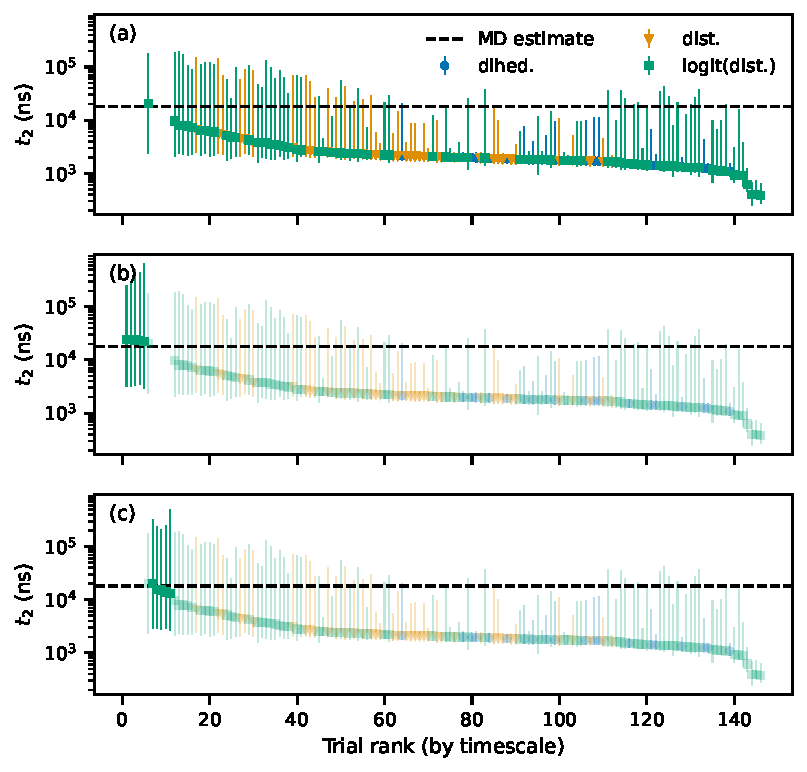
\includegraphics[width=0.8\textwidth]{figures/1fme_timescales.pdf}
    \caption{Slowest timescale $t_{2}$ extracted from each trial MSM. Panel (a) shows the randomly sampled hyperparameter trials. Panel (b) includes the results of one iteration of Bayesian optimisation (original trials shown as transparent). Panel (c) includes the results of one iteration of Bayesian optimisation excluding the influence of the best ranked trial in panel (a).  Central value and error bars are derived from 100 bootstrap samples as the median, the \SI{95}{\percent} quantiles. The blacked dashed line is the value  reported in~\cite{lindorff-larsen_how_2011} and is derived directly from the MD trajectories.} 
    \label{fig:1fme_timescales}
\end{figure}

Figure \ref{fig:1fme_timescales} show the slowest timescale extracted from each of the MSMs. The value determined from analysis of the MD trajectories~\cite{lindorff-larsen_how_2011} is \SI{18}{\micro\second} and is shown as a dashed line. Only a single set of hyperparameters predicts a timescale close to this value (\SI{20}{\micro\second}, unsigned error: \SI{14}{\percent}), while the other trials an unsigned error of  at least \SI{45}{\percent}. The trials using the logistic-distances (soft-contact map) make up the majority of both the best and worst performing hyperparameters; while the dihedral and contact distances sit within the middle of the distribution of timescales (see figure~\sref{fig:ts_distribution}). This suggests that only a small volume of the hyperparameter search space gives rise good models.  


\subsection{How sensitive are timescales to the MSM hyperparameters?}\label{sec:sensitivity}

\begin{figure}
    \centering
    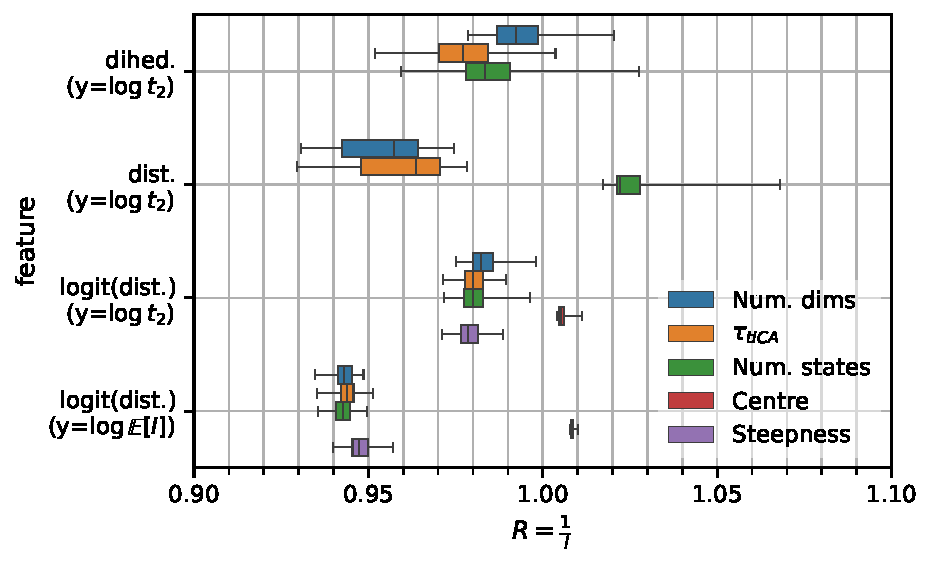
\includegraphics[width=0.8\textwidth]{figures/sensitivity.pdf}
    \caption{Hyperparameter relevance ($R$) to the timescales ($y=\log{t_{2}}$)for the three different features,  and the expected improvement ($y=\log{\mathbb{E}[I]}$) for the logistic-distances feature. The larger the relevance, the more sensitive the outcome is to each hyperparameter.  The relevance is calculated from the learned kernel parameters of the relevant Gaussian process. Box plots show the distribution of values from \num{100} bootstrap samples. The relevance $R$ is the inverse of the characteristic length-scale of the exponential kernel in equation xxx. }
    \label{fig:sensitivity}
\end{figure}

In order to understand the sparsity of good hyperparameters we estimate the sensitivity of the timescales to the hyperparameters. Previous work has shown that the type of feature used is important in determining the eigenvector accuracy. This is consistent with figures~\ref{fig:1fme_timescales}  where the majority of the best hyperparameters use the soft-contact map (logistic distances) feature.  However, as figure~\ref{fig:ts_distribution} also shows that a) there is significant overlap of the timescale distributions for each feature, and b) the best performing feature also gives rise to the worst performing models. The type of feature is therefore a necessary but not sufficient hyperparameter to tune in order to maximize the timescales. It is important, therefore, to consider the remaining hyperparameters (e.g., the TICA lag time, TICA dimension etc.) and how they affect the timescales.  

We estimate the sensitivity of the remaining hyperparameters for each feature by modelling $\log{t_{2}} \sim \mathcal{GP}(\bm{mu}, \mathbf{K})$. This model of the response of the $t_2$ to variation in the hyperparameters we call a \emph{response surface}. The elements of $\mathbf{K}$ were given by equation~\ref{eqn:kernel}, and $\bm{\theta} = (m, \tau, n)$  for the dihedral feature,  $\bm{\theta} = (d, m, \tau, n)$ for the linear distances feature, and $\bm{\theta} = (d m, \tau, n, c, s)$  for the logistic distances feature. An exponential kernel in $\mathbf{K}$ gave the best fitting model as judged by the RMSE. The sensitivity is calculated from the characteristic length-scales, $l$, in $\mathbf{K}$ via the relevance $R=1/l$.  

Figure~\ref{fig:sensitivity} plots the  the relevance of hyperparameters, $R$, in determining $t_{2}$. It shows that the hyperparameters vary in how important they are in determining $t_2$ for each different feature.  For the dihedral feature (`dihed.') its shows that the TICA dimension, lag time and number of microstates are all equally relevant in determining $t_2$, however $t_2$ does not vary greatly with changes in any of these hyperparameters (as $R\simeq 1$). For the inter-residue distance feature (`dist.') the number of microstates is the most relevant in determining $t_2$. For the logistic-distances feature (`logit(dist.)') the location of the centre of the logistic function (which corresponds approximately to the contact map cut-off) is the most important hyperparameter. The fitted Gaussian process regression models which give rise these values are shown in the supplementary material figures~\ref{fig:repsonse_diheds}, \ref{fig:repsonse_dist}, and \ref{fig:repsonse_logistic}. 

Why is the hyperparameter sensitivity important? As was previously shown~\cite{bergstra_jamesbergstra_random_2012} if all the hyperparameters have a large relevance ($R \gg 1$) then to find the maximum of the response surface (i.e., the hyperparameters which give rise to the maximim $t_2$) then it is important to try all combinations of hyperparameters i.e., a  grid-search strategy, or to employ an active learning approach~\cite{snoekAbstractBayesianOptimization2013}.  However, if only a small proportion of the hyperparameters have a high relevance then randomly sampling hyperparameters is the more efficient strategy. 

\subsection{Can we improve the timescale estimates?}

\begin{figure}
    \centering
    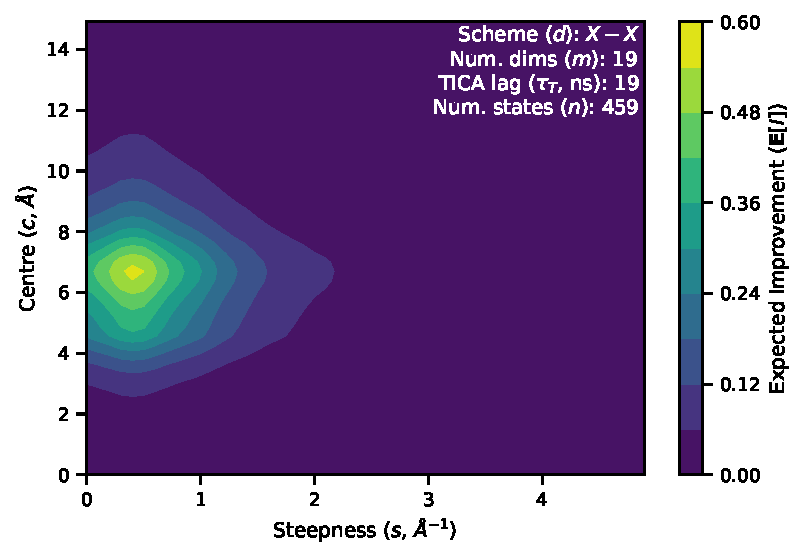
\includegraphics{figures/surface_distances_logistic_ei.pdf}
    \caption{Expected improvement as a function of the two most relevant hyperparameters - the logistic center ($c$) and steepness ($s$). The remaining hyperparameters take on the values shown in the annotation. These were chosen so as to maximize the expected improvement, i.e., the figure plots $y=f(s, c, d^{*}, m^{*}, \tau^{*}, n^{*})$ where $s^{*}, c^{*}, d^{*}, m^{*}, \tau^{*}, n^{*} = \argmax \left [f(s, c, d, m, \tau,n)\right]$. }
    \label{fig:ei_surface}
\end{figure}

In order to check the convergence of the results shown in panel (a) of figure~\ref{fig:1fme_timescales} and to potentially improve the $t_2$ estimate,  we use a single round of Bayesian optimisation. To do this, we first calculate the expected improvement, $\mathbb{E}[I]$,  using the response surface calculated previous using equation~\ref{eqn:ei_for_gp} for the logistic distances feature only. We then estimated MSMs using the five sets of hyperparameters with the largest expected improvement. The details of this procedure can be found in the supplementary materials. 

In the previous section we determined what hyperparameters were most relevant for determining the dominant timescale, $t_2$, for the logistic distances feature this was centre of the logistic curve. Similarly, we can ask: what are the most relevant hyperparameters for the expected improvement?  This is shown in figure~\ref{fig:sensitivity} (`logit(dist.)', $y=\mathbb{E}[I]$) which shows the `centre' hyperparameter is  most important but by a larger margin compared to the other hyperparameters.  The expected improvement is shown in figure~\ref{fig:ei_surface} as a function of the `centre' and the `steepness' hyperparameters (the remaining hyperparameters are held at their values at the peak of expected improvement).  This shows that we expect any values of the `centre' and `steepness' hyperparameters to increase $t_2$ by at least \SI{2}{\micro\second} if the other hyperparameters take on their values in the annotation. However, with $c\simeq \SI{7}{\angstrom}$ and $s\simeq \SI{0.5}{\per\angstrom}$ we can expect an improvement in the timescales of almost $\SI{3}{\micro\second}$. 

The new optimized values of $t_2$ are shown in panel (b) of figure~\ref{fig:1fme_timescales}.  These clearly show that optimized models all have timescales slightly greater than the incumbent (the best timescale before the optimisation, shown in purple, with $t_2 \simeq \SI{20}{\micro\second}$):  the optimised timescales range up to $t_2 \simeq \SI{24}{\micro\second}$, which are similar to the improvements predicted by the expected improvement function. The optimised hyperparameters differ slightly from the incumbent (except in the choice of distance scheme - all used the alpha-carbon distances). We have, therefore, a set of six MSMs which differ slightly in the values of their hyperparameters, which all give similar implied timescales: we can be sure that our model is robust. 

We can also ask ourselves whether we could improve our hyperparameters using Bayesian optimisation with less data. This is relevant if estimating the models is expensive. To answer this we remove the incumbent in panel (b) from the hyperparameter trial data-set, re-estimate the response surface and expected improvement and sample new hyperparameters. The new incumbent in this case is $t_2 = \simeq \SI{10}{\micro\second}$, shown in purple in panel (c) figure~\ref{fig:1fme_timescales}.  The new values of $t_2$,  are all improvements of up to \SI{10}{\micro\second} the new timescales range up to $t_2 \simeq \SI{20}{\micro\second}$. It is therefore plausible that one may use Bayesian optimisation to optimise MSM hyperparameters, even when the timescale measurements are noisy and there are no strong dependence on any of hyperparameters.  



\subsection{Are VAMP scores suitable for model selection of reversible MSMs?}
\begin{figure}
    \centering
    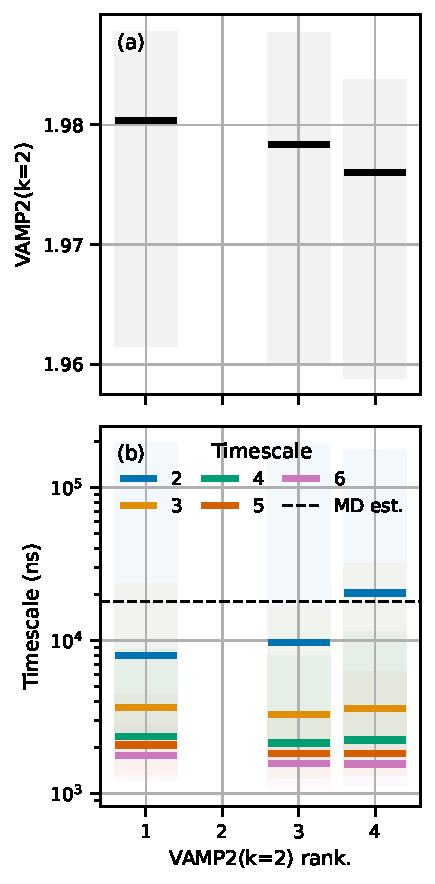
\includegraphics{figures/bad_vamp_ranks.pdf}
    \caption{Models with VAMP scores inversely proportional to timescales. Panels (a) and (c) show the VAMP2 scores (as calculated by equation~\ref{eqn:vamp_score_def} and as implemented in the package Deeptime~[ref]) for a selection of models where the slowest timescale is inversely proportional to the VAMP2(k=2) score. The horizontal axis is the model rank as judged by the VAMP2(k=2) score. Models which do not show this correlation are not shown.  Panels (b) and (d) show similar but for a lower ranking set of models. }
    \label{fig:bad_vamp_scores}
\end{figure}


\begin{figure}
    \centering
    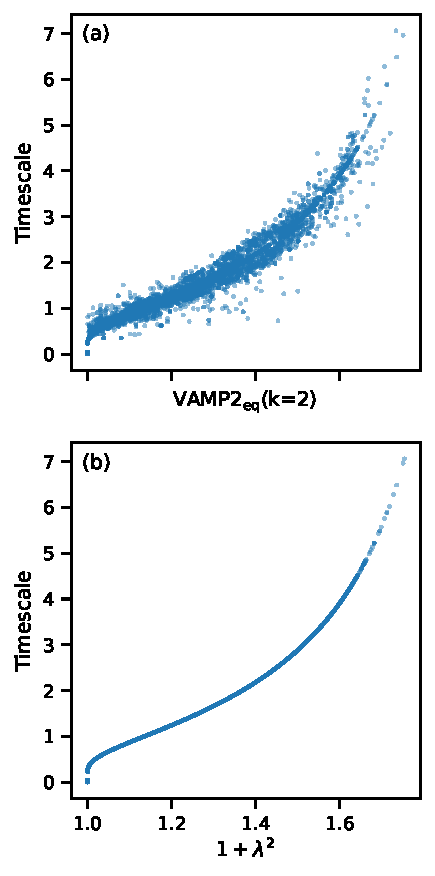
\includegraphics{figures/timescale_vs_vamp_vs_evs.pdf}
    \caption{Timescales as a function of the VAMP2 scores (panel (a) and sum of square eigenvalues (b). Each point is calculated from a simulated trajectory of 20 observations using the $3\times 3$ example in Trendelkamp-Schroer et. al.~\cite{trendelkamp-schroerEstimationUncertaintyReversible2015b}. The transition matrix was estimated ensuring reversibility, all calculations were performed using the Deeptime package. There are 10000 points in total.}
    \label{fig:bad_vamps_examples}
\end{figure}


The VAMP2 score~\cite{wuVariationalApproachLearning2020c} provide a principled metric for optimising MSM hyperparameters. The benefits are that it can be used for stationary, non-stationary, reversible and non-reversible MSMs. It is linked directly to the kinetic variance captured by the basis states such that maximizing the VAMP2(k) score will maximize the timescales of pertaining to the first $k$ eigenvectors of the model. In addition it can be used with bootstrapping and cross-validation model selection techniques. 

We tested whether the VAMP scores are appropriate for model selection with reversible MSMs. For each of the hyperparameters trials we calculated the VAMP2(k=2) score so that we are focused solely on maximizing the dominant $t_2$ timescale. Inspection of the results revealed that for subsets of the trials, VAMP2(k=2) was inversly proportional to the $t_2$. This is shown in figure~\ref{fig:bad_vamp_scores}. In panel (a) the VAMP2 score is shown for the trials ranked first, third, and fourth. In panel (c) the first five timescales are shown for each model.  The dashed line shows the folding timescale from reference~\cite{lindorff-larsen_how_2011}. Timescales for the third to sixth eigenvectors are the same, however $t_2$ clearly \emph{increases} with \emph{decreasing} VAMP2 score. The second ranked model is omitted for clarity because it does not follow this pattern. 

We posit that the reason for this behaviour is due to the fact by enforcing reversibility in the estimation of the transition matrix it is impossible to get consistency between the three count matrices ($\mathbb{C}_{00, 0t, tt}$) and the eigenvectors ($\mathbb{U}/\mathbb{V}$) in equation~\ref{eqn:vamp_score_def}).  A similar effect can be seen with a three-state toy model (example 1 from~\cite{trendelkamp-schroer_estimation_2015}). \num{10000} 20-step trajectories were sampled from the same transition matrix. The implied timescales and VAMP2(k=2) scores were estimated and are shown in figure ~\ref{fig:bad_vamps_examples} panel (a).  The timescales are correlated with the VAMP2 scores but the correlation is not perfect. Many subsets of these results could form sets which are anti-correlated, in the same way as in figure~\ref{fig:bad_vamp_scores}. In panel (b) we plot the sum of the squares of the first two eigenvalues, which shows perfect rank correlation (as they must as they are analytically related to each other). 

The reason for writing the VAMP score as the product of count  matrices and eigenvectors/singular vector matrices is to facilitate data-splitting in cross-validation. While we used bootstrapping for this work, the effect of data splitting would be to worsen the discrepancy between the count and transition matrices. This is because the count matrices are now estimated on different data compared to the eigenvector matrices.  


In addition to the problem of consistency between the matrices in equation~\ref{eqn:vamp_score_def} from a) enforcing reversibility and b) data splitting for cross-validation, we recommend that cross-validated VAMP scores are not used for reversible and stationary MSMs.  Instead we recommend bootstrapping the sum of the squared eigenvalues (VAMP$_{eq}$(k)) directly from the reversible transition matrix. This has the same theoretical properties of the VAMP2 score (i.e., represents captured kinetic variance, and link to variational theorem) while not wasting data due to data splitting and perfect correlation with the implied timescales. 

\subsection{Does the lag time and number of scored eigenvectors affect the model selection?}

\begin{figure}
    \centering
    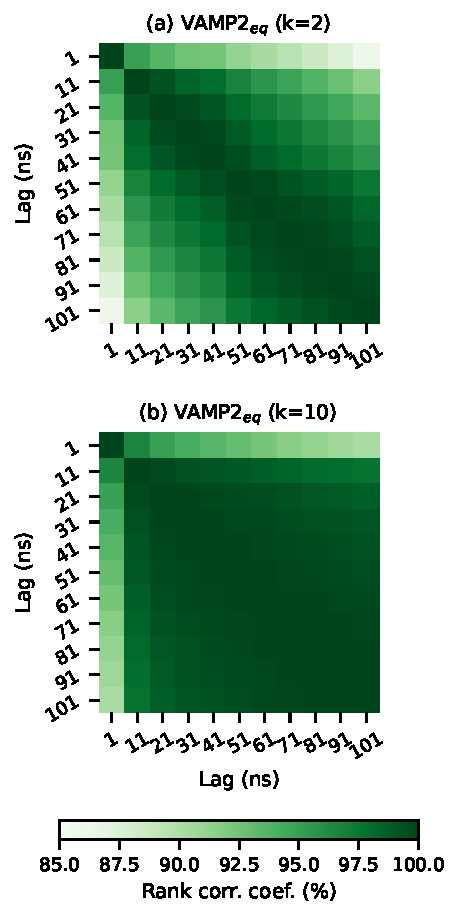
\includegraphics{figures/vampeq_rank_vs_lag.pdf}
    \caption{Consistency of $\operatorname{VAMP2}_{\mathrm{eq}}(k)=\sum_{i=1}^{k}\lambda_{i}^{2}$ rank with Markov lag time, $\tau$. The $i, j$'th cell in panel (a) shows the Spearman's rank correlation coefficient of $\operatorname{VAMP2}_{\mathrm{eq}}(k=2)$ for each trial measured at the $i$'th lag time, with   $\operatorname{VAMP2}_{eq}(k=2)$  measured at the $j$'th lag time.  Only the top $50$ trials as measured at the $i$th lag time were used.  Panels (b) - (d) show the same measurements but with $k=3, 5$ and $10$  in the $\operatorname{VAMP2}_{\mathrm{eq}}(k)$ score respectively. }
    \label{fig:vamp_rank_vs_lag}
\end{figure}

When evaluating MSMs using a variational score one must specify the both the Markov lag time ($\tau$) and the number of eigenvectors to score ($k$).  However, both these choices affect the VAMP scores although it is not clear  whether these choices affect the model ranking.  To test how these choices affect model selection we measured the consistency in model rank, as measured by the VAMP2$_{eq}$(k) using the Spearman's rank correlation coefficient, at a) different lag times for given values of $k$ and b) at different numbers of scored eigenvector at a given lag time. 


Figure~\ref{fig:vamp_rank_vs_lag} shows the consistency between model rankings at different lag times ($\SI{1}{\nano\second} < \tau < \SI{101}{\nano\second}$) with $k=2$ (panel (a)) and with $k=10$ (panel (b)). In addition, scatter plots of the data used to calculate these coefficients for $k=2, 3, 5, \& 10$ are shown in the supplementary information figures~\ref{fig:vampeq2_rank_vs_lag_pairplot} to \ref{fig:vampeq10_rank_vs_lag_pairplot}.  Across all lags and for both small and large numbers of scored eigenvectors, the consistency in the model ranking is high (greater than \SI{85}{\percent}). For all but the shortest lag time ($\tau=\SI{1}{\nano\second}$) the rank correlation is much greater, ranging up to \SI{100}{\percent} for between long lag-times.  this effect is most pronounced for larger numbers of scored eigenvectors. In particular, good consistency is achieved at lag times smaller than those required for the model to be Markovian ($\tau=\SI{41}{\nano\second}$).


\begin{figure}
    \centering
    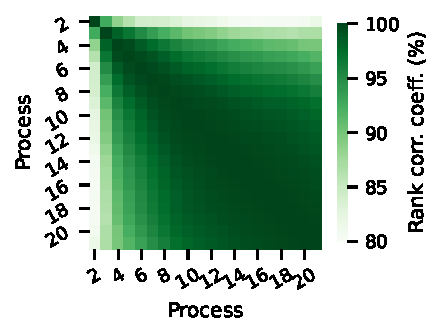
\includegraphics{figures/vampeq_rank_vs_proc.pdf}
    \caption{\textsc{Consistency of $\operatorname{VAMP2}_{eq}(k)$ rank with number of scored eigenvectors}. The ranks of trials in the row $k$ are compared to their rank at the column $k$ using the Spearman's rank correlation coefficient at a lag time of \SI{41}{\nano\second}}
    \label{fig:vampeq_rank_vs_n_procs}
\end{figure}

Figure~\ref{fig:vampeq_rank_vs_n_procs} shows the consistency between model rankings at different number of scored eigenvectors ($2 < k < 21$) at a lag time of \SI{41}{\nano\second} (the value used in all previous analysis). Again, the consistency is generally high with a rank correlation between all pairs of $k$ of at least \SI{80}{\percent}. The ranking is most consistent between values of $k$ larger than \num{4}.  From these two analyses taken together, we see that for long lag-times and large number of scored eigenvectors model ranking is not affected by the choice of $\tau$ and $k$.


\subsection{Conclusions}
This work has answered a number of questions pertaining to selecting hyperparameters for discrete MSMs.  We have seen that type of feature is important but that the other hyperparameters need to be chosen carefully to optimise the implied timescales.  The sensitivity of the implied timescales is generally low, meaning small variations in their values do not change the timescales significantly.  However, the relative sensitivity of the non-feature hyperparameters changes depending on type of feature used: e.g., with some features the number of microstates is most important while with others the timescales are not affected.  The VAMP variational scores, which have recently used to perform model selection on reversible MSMs have been shown to give results which are not in line with the variational principle underlying them. 

Given this relatively complex picture of hyperparameter optimisation we recommend the following for optimising reversible MSMs: 

\begin{enumerate}
    \item A number of different features should be tried. They can be selected from a list, potentially informed by the VAMP scores developed for by Schrere et. al. \cite{scherer_variational_2019}. 
    \item Remaining hyperparameters should be randomly sampled from a suitable search space. Using a grid search method is inefficient and not easily modified to sample more hyperparameter if necessary. 
    \item Scoring models using bootstrapped values of sum of squared eigenvalues is preferable to using the VAMP2 variational score because it can lead to contradictory results. 
    \item If the MSM requires significant resources, Bayesian optimisation may be a useful tool.  This work used a Gaussian process surrogate model but other, more flexible models may perform better (see limitations discussion below). 
    \item Even if the the MSM does not require significant resources, Bayesian optimisation provides a principled way of checking the convergence the model.  We suggest reporting an optimised model and a set of models which make it clear that the behaviour of model observables is consistent with varation in the hyperparmeters. 
    \item When scoring the models use as many eigenvectors as are resolvable. This can be estimated from a selection of models or all processes can be scored and saved in a database (as was performed here).  
    \item For model selection, it is not important to select a `Markovain' lag time although this should be attempted to be estimated from a selection of models.  
\end{enumerate}

There are a number of limitations to this study.  First the we have a performed our analysis on only one system which limits the applicability some of the specific results. For example, the sensitivity of the hyperparameters to the timescales should be not taken as generally applicable for other systems. Second, the fitting of the Gaussian process used in the sensitivity calculation and the Bayesian optimisation required a lot of ad-hoc preprocessing and its own model selection procedure.  More flexible models which still return estimates of input importance and of uncertainty, such as random forests or tree parzen estimators, may be more appropriate.  Third, it is 


\subsection{References}



%%%%%%%%%%%%%%%%%%%%%%%%%%%%%%%%%%%%%%%%%%%%%%%%%%%%%%%%%%%%%%%%%%%%%
%% The "Acknowledgement" section can be given in all manuscript
%% classes. This should be given within the "acknowledgement"
%% environment, which will make the correct section or running title.
%%%%%%%%%%%%%%%%%%%%%%%%%%%%%%%%%%%%%%%%%%%%%%%%%%%%%%%%%%%%%%%%%%%%%
\begin{acknowledgement}

Please use ``The authors thank \ldots'' rather than ``The
authors would like to thank \ldots''.


\end{acknowledgement}

%%%%%%%%%%%%%%%%%%%%%%%%%%%%%%%%%%%%%%%%%%%%%%%%%%%%%%%%%%%%%%%%%%%%%
%% The same is true for Supporting Information, which should use the
%% suppinfo environment.
%%%%%%%%%%%%%%%%%%%%%%%%%%%%%%%%%%%%%%%%%%%%%%%%%%%%%%%%%%%%%%%%%%%%%
\begin{suppinfo}


\end{suppinfo}

%%%%%%%%%%%%%%%%%%%%%%%%%%%%%%%%%%%%%%%%%%%%%%%%%%%%%%%%%%%%%%%%%%%%%
%% The appropriate \bibliography command should be placed here.
%% Notice that the class file automatically sets \bibliographystyle
%% and also names the section correctly.
%%%%%%%%%%%%%%%%%%%%%%%%%%%%%%%%%%%%%%%%%%%%%%%%%%%%%%%%%%%%%%%%%%%%%
\bibliography{references.bib}

\end{document}





% \begin{itemize}
    % \item Markov state models are a popular model for analysing MD data. 
    % \item They are able to provide a quantitative picture of the conformational dynamics of biomolecular systems. 
    % \item They have been used to study protein folding, ligand binding, peptide- and protein-protein association,  enzymatic reaction dynamics. 
    % \item They have also been used in adaptive sampling algorithms where statistical properties of the model are used to select conformations from which to seed more MD simulations to speed convergence. 
    % \item Like any any statistical model, a number of choices must be made when estimating an MSM. These include choice of estimation algorithm, convergence criteria for optimizing loss-functions; batching, sub-sampling and splitting data for compute resource management and estimating out of sample accuracy; data pre-processing e.g., image resizing, feature-scaling and warping; feature selection and egineering, de-correlating etc. 
    % % \item These choices affect the outcome of the model to varying to degrees but are not `learned' from the data via minimizing a loss function, in the way the parameters of the model are (e.g., neural network weights, MSM transition matrix elements). For this reason they are called `hyperparameters' of the model. 
    % \item There has been a lot of recent attention paid to the affects of hyperparameter selection in, for e.g.,  psychology, neuroscience and machine learning  where opaque methods of hyperparameter selection have lead to irrepreducible results. 
    % \item There are a host of different approaches to this problem, which differ according to whether explanatory power or predictive accuracy of the model are required. 
    % \item When statistical models are made for their explanatory power variants of sensitivity analysis are often used. SA entails estimating models with  several plausible sets of hyperparameters to see how they affect the results [ref].  Similarly, multiverse analysis uses a more thorough enumeration of potential hyperparameters [ref].  Specification curve analysis [ref] also uses a multiverse of results while going further to infer information from the distribution of results. 
    % \item In machine learning, where predictive power is often more important, hyperparameters can be chosen to optimize performance metrics of the model, e.g., out of sample accuracy. Hyperparameters can be randomly or uniformly selected, or even optimized using e.g., Bayesian optimisation.  
    % \item The essential task in MSM estimation is to choose hyperparameters for preprocessing MD data into a smaller number of basis  states for which the MSM can be estimated. 
    % \item traditionally these basis states are discrete states corresponding to small regions of configuration space of the protein. Recent work has focused on estimating fuzzy basis sates using deep learning approaches.  
    % \item Either way a number of hyperparameters must be chosen. The resulting basis states can be judged according to variational scores. 
    % \item For reversible MSMs the generalized matrix Rayleigh coefficient (GMRQ) was introduced as metric of optimising basis states.  This was later expanded to include non-reversible and non-stationary MSMs with the variational approach to Markov processes (VAMP). 
    % \item By varying hyperparameters to increase the variational score, the basis states can be made increasingly accurate. 
    % \item  However, most recent papers which utilise MSMs as their man analytic tool, do not report how hyperparameters were chosen.  
    % \item Where methods for hyperparameter selection were discussed VAMP scores were generally used to discriminate between a handful of different hyperparameters.  
    % \item Taking inspiration from the literature on sensitivity analysis and hyperparameter optimisation we investigate whether more extensive hyperparameter selection methods are needed or appropriate. 
    % \item We investigate how sensitive how MSM timescales are to changes in hyperparameters, demonstrate how an active learning approach might work to finding good quality hyperparameters might work and comment on the commonly used VAMP scores for optimizing basis states.
    % \item This work is structured as follows. Section~\ref{theory} covers the theory of Markov state models and of hyperparameter optimisation and search strategies; section~\ref{methods} covers the methods and materials used; section~\ref{results} discusses results using the fast folding protein BBA as an example; section~\ref{conclusion} concludes with recommendations for estimating MSMs. 
% To get a sense of the current practice for estimating MSMs a small survey of recent literature was conducted. Web Of Science[] was used to look for articles citing PyEMMA~\cite{schererPyEMMASoftwarePackage2015a}, Enspara~\cite{porter_enspara_2019} and MSMBuilder~\cite{beauchamp_msmbuilder2:_2011} and Deeptime~\cite{deeptime}, published since 2020 and 25 randomly selected for detailed investigation~\cite{tosstorff_study_2020, fernandez-quintero_mutation_2021, kahler_sodium-induced_2020, paul_thermodynamics_2021, quoika_implementation_2021, liu_misfolding_2020, tian_deciphering_2020, hempel_molecular_2021, koulgi_structural_2021., sharma_comparative_2020, mckiernan_dynamical_2020, dutta_distinct_2022, zhou_molecular_2021, fernandez-quintero_cdr_2022, song_modulation_2021, sadiq_multiscale_2021, ibrahim_dynamics_2022, linker_polarapolar_2022, hu_discovery_2022, cannariato_prediction_2022, jones_determining_2021, zhu_critical_2021, zhu_critical_2021, bergh_markov_2021, pantsar_decisive_2022, grabski_molecular_2021}. Articles looking at purely methodological questions were excluded. Three questions were asked: 
% \begin{itemize}
%     \item Were sensitivity analyses performed? i.e., were the sensitivity of observables tested with respect to the model hyperparameters?
%     \item How did the authors select the hyperparameters? e.g., using VAMP score? 
%     \item Did the authors perform a validation of the selected model using implied timescales and/or a Chapman-Kolmogorov test? 
% \end{itemize}

% Only one of the studies presented a sensitivity analysis, (this analysis also served as a hyperparameters selection technique)~\cite{bergh_markov_2021}. The the majority (15, \SI{60}{\percent}) of studies did not discuss any hyperparameter search techniques and of those that did,  the majority~\cite{paul_thermodynamics_2021, koulgi_structural_2021, sharma_comparative_2020, dutta_distinct_2022, zhou_molecular_2021, jones_determining_2021, zhu_critical_2021, grabski_molecular_2021} used VAMP scores (8, \SI{89}{\percent}), while one article used the elbow method with important observables \cite{bergh_markov_2021} as their objective function. Only a minority~\cite{quoika_implementation_2021, hempel_molecular_2021, song_modulation_2021, ibrahim_dynamics_2022} failed to give evidence of validation.  

% It can be concluded that hyperparameter optimisation is popular but not universal and sensitivity analysis is either a) not performed or b) not thought important (either by journals or by the authors) enough not to include in the journal article. 
% \end{itemize}





% \begin{itemize}
%     \item The variational theorem applied to the transfer operator $\mathcal{T}(\tau)$, implies that the sum eigenvalues of the $\mathbf{T}$ in some arbitrary basis, will always be less than the sum of the true eigenvalues. 
%     \item Thus, one is free to choose a basis which will increase the sum of the eigenvalues. The associated timescales and eigenvectors will become closer to the true timescales and eigenvectors. 
%     \item In practice we restrict the score to pertain to the $k$ slowest processes, where $k=2 - \simeq 10$. We write the score as $S(\bm{\theta}; k) = \sum_{i=1}^{k}\lambda_{i}$. The functional dependence on $\bm{\theta}$ highlights the fact that the score is assessing the accuracy of the basis states. 
%     \item A general method of finding the most accurate basis states would be to vary the elements of $\bm{\theta}$ until a sufficiently large value of $S$ is found.  However, as pointed out in [mcgibbon] this would favour basis states which fit to noisy fluctuations in the data and do not represent the most accurate basis states, i.e., they would over-fit to the data at hand.
%     \item There are two common techniques to avoid over-fitting. First is the Bootstrap [ref bootstrap] and Cross-validation. The approach  taken by [Noe] and [Pande] is to use cross-validation. 
%     \item The cross-validated estimator of $S$ first estimates the eigenvectors on half of the discretized MD data (the matrix of eigenvectors is given by $\mathbf{U}^{i}$, where the $i$ denotes the $i$th training cross-validation split) the count ($\mathbf{C}_{01}^{-i}$, where $-i$ denotes the complementary test split to $i$) and population ($\mathbf{C}_{00}^{-i}$) matrices are estimated on the remaining half of the data. This is repeated $N$ times with the score being given by: 
%     \begin{equation}
%         GMRQ(\bm{\theta}; k) = \frac{1}{N}\sum_{i}^{N} \operatorname{Tr}\left[(\mathbf{U}^{iT}\mathbf{C}_{01}^{-i}\mathbf{U}^{i})(\mathbf{U}^{iT}\mathbf{C}_{00}^{-i}\mathbf{U}^{i})^{-1}\right]
%     \end{equation}\label{eqn:gmrq_cv_def}
%     \item In other words, this tests how well the training eigenvectors, diagonalize the test count and population matrices. 
%     \item Because the eigenvectors are estimated from a reversible transition matrix they are not consistent with the count matrix.  To account for this, a symmetrized count matrix is used: $\mathbf{C}_{01}^{\mathrm{rev}} = \mathrm{T}^{\mathrm{rev}}\cdot \bm{\Pi}^{\mathrm{rev}}$.  Where $\Pi$ is a diagonal matrix with the elements of $\pi$ on its diagonal. 
%     \item The VAMP scores follow the same principle as the GMRQ but with a distinction drawn between populations at time $t$ and at time $t+\tau$. I.e., $\mathbf{C}_{00} \neq \mathbf{C}_{11}$
%     \item this is to allow the possibility of non-stationary and non-reversible models.
%     \item Instead of eigenvectors, left and right singular vectors, $\mathbf{U}$ and $\mathbf{V}$ of the transition matrix are used (the cross-validation notation is dropped for clarity): 

%     \item When the count and population matrices and the singular vectors are all estimated from the same data, this amounts to the sum of the singular vectors raised to the power of $r$.  
%     \item When $\mathbf{C}_{00} = \mathbf{C}_{11}$ and $\mathbf{C}_{01}$ symmetric, then this expression with $r=1$ should be equivalent to the GMRQ.  i.e., the singular values should equal the eigenvalues.  
%     \item With $r=2$ this expression measures the kinetic variance~\cite{noeKineticDistanceKinetic2015} captured by the basis sets. 
%     \item Both scores truncate the eigenvector/singular vectors to the first $k$ components to restrict the score to just those processes. 
%     \item Both formulae can also be used with bootstrapping where the train and test data are the same but $N$ datasets are generated by sampling with replacement from the pool of available MD trajectories.   
%     \item The VAMP-r scores have also been adapted to score the features only [ref]. 
% \end{itemize}